%% bare_jrnl.tex
%% V1.4b
%% 2015/08/26
%% by Michael Shell
%% see http://www.michaelshell.org/
%% for current contact information.
%%
%% This is a skeleton file demonstrating the use of IEEEtran.cls
%% (requires IEEEtran.cls version 1.8b or later) with an IEEE
%% journal paper.
%%
%% Support sites:
%% http://www.michaelshell.org/tex/ieeetran/
%% http://www.ctan.org/pkg/ieeetran
%% and
%% http://www.ieee.org/

%%*************************************************************************
%% Legal Notice:
%% This code is offered as-is without any warranty either expressed or
%% implied; without even the implied warranty of MERCHANTABILITY or
%% FITNESS FOR A PARTICULAR PURPOSE! 
%% User assumes all risk.
%% In no event shall the IEEE or any contributor to this code be liable for
%% any damages or losses, including, but not limited to, incidental,
%% consequential, or any other damages, resulting from the use or misuse
%% of any information contained here.
%%
%% All comments are the opinions of their respective authors and are not
%% necessarily endorsed by the IEEE.
%%
%% This work is distributed under the LaTeX Project Public License (LPPL)
%% ( http://www.latex-project.org/ ) version 1.3, and may be freely used,
%% distributed and modified. A copy of the LPPL, version 1.3, is included
%% in the base LaTeX documentation of all distributions of LaTeX released
%% 2003/12/01 or later.
%% Retain all contribution notices and credits.
%% ** Modified files should be clearly indicated as such, including  **
%% ** renaming them and changing author support contact information. **
%%*************************************************************************


% *** Authors should verify (and, if needed, correct) their LaTeX system  ***
% *** with the testflow diagnostic prior to trusting their LaTeX platform ***
% *** with production work. The IEEE's font choices and paper sizes can   ***
% *** trigger bugs that do not appear when using other class files.       ***                          ***
% The testflow support page is at:
% http://www.michaelshell.org/tex/testflow/



% \documentclass[conference,final]{IEEEtran}
%
% If IEEEtran.cls has not been installed into the LaTeX system files,
% manually specify the path to it like:
% \documentclass[journal]{../sty/IEEEtran}

% \usepackage[utf8]{inputenc}



% Some very useful LaTeX packages include:
% (uncomment the ones you want to load)


% *** MISC UTILITY PACKAGES ***
%
%\usepackage{ifpdf}
% Heiko Oberdiek's ifpdf.sty is very useful if you need conditional
% compilation based on whether the output is pdf or dvi.
% usage:
% \ifpdf
%   % pdf code
% \else
%   % dvi code
% \fi
% The latest version of ifpdf.sty can be obtained from:
% http://www.ctan.org/pkg/ifpdf
% Also, note that IEEEtran.cls V1.7 and later provides a builtin
% \ifCLASSINFOpdf conditional that works the same way.
% When switching from latex to pdflatex and vice-versa, the compiler may
% have to be run twice to clear warning/error messages.






% *** CITATION PACKAGES ***
%
% \usepackage{cite}
% cite.sty was written by Donald Arseneau
% V1.6 and later of IEEEtran pre-defines the format of the cite.sty package
% \cite{} output to follow that of the IEEE. Loading the cite package will
% result in citation numbers being automatically sorted and properly
% "compressed/ranged". e.g., [1], [9], [2], [7], [5], [6] without using
% cite.sty will become [1], [2], [5]--[7], [9] using cite.sty. cite.sty's
% \cite will automatically add leading space, if needed. Use cite.sty's
% noadjust option (cite.sty V3.8 and later) if you want to turn this off
% such as if a citation ever needs to be enclosed in parenthesis.
% cite.sty is already installed on most LaTeX systems. Be sure and use
% version 5.0 (2009-03-20) and later if using hyperref.sty.
% The latest version can be obtained at:
% http://www.ctan.org/pkg/cite
% The documentation is contained in the cite.sty file itself.






% % *** GRAPHICS RELATED PACKAGES ***
% %
% \ifCLASSINFOpdf
%   \usepackage[pdftex]{graphicx}
%   % declare the path(s) where your graphic files are
%   % \graphicspath{{../pdf/}{../jpeg/}}
%   % and their extensions so you won't have to specify these with
%   % every instance of \includegraphics
%   \DeclareGraphicsExtensions{.pdf,.jpeg,.png}
% \else
%   % or other class option (dvipsone, dvipdf, if not using dvips). graphicx
%   % will default to the driver specified in the system graphics.cfg if no
%   % driver is specified.
%   % \usepackage[dvips]{graphicx}
%   % declare the path(s) where your graphic files are
%   % \graphicspath{{../eps/}}
%   % and their extensions so you won't have to specify these with
%   % every instance of \includegraphics
%   % \DeclareGraphicsExtensions{.eps}
% \fi
% % graphicx was written by David Carlisle and Sebastian Rahtz. It is
% % required if you want graphics, photos, etc. graphicx.sty is already
% % installed on most LaTeX systems. The latest version and documentation
% % can be obtained at: 
% % http://www.ctan.org/pkg/graphicx
% % Another good source of documentation is "Using Imported Graphics in
% % LaTeX2e" by Keith Reckdahl which can be found at:
% % http://www.ctan.org/pkg/epslatex
% %
% % latex, and pdflatex in dvi mode, support graphics in encapsulated
% % postscript (.eps) format. pdflatex in pdf mode supports graphics
% % in .pdf, .jpeg, .png and .mps (metapost) formats. Users should ensure
% % that all non-photo figures use a vector format (.eps, .pdf, .mps) and
% % not a bitmapped formats (.jpeg, .png). The IEEE frowns on bitmapped formats
% % which can result in "jaggedy"/blurry rendering of lines and letters as
% % well as large increases in file sizes.
% %
% % You can find documentation about the pdfTeX application at:
% % http://www.tug.org/applications/pdftex





% % *** MATH PACKAGES ***
% %
% %\usepackage{amsmath}
% % A popular package from the American Mathematical Society that provides
% % many useful and powerful commands for dealing with mathematics.
% %
% % Note that the amsmath package sets \interdisplaylinepenalty to 10000
% % thus preventing page breaks from occurring within multiline equations. Use:
% %\interdisplaylinepenalty=2500
% % after loading amsmath to restore such page breaks as IEEEtran.cls normally
% % does. amsmath.sty is already installed on most LaTeX systems. The latest
% % version and documentation can be obtained at:
% % http://www.ctan.org/pkg/amsmath





% % *** SPECIALIZED LIST PACKAGES ***
% %
% %\usepackage{algorithmic}
% % algorithmic.sty was written by Peter Williams and Rogerio Brito.
% % This package provides an algorithmic environment fo describing algorithms.
% % You can use the algorithmic environment in-text or within a figure
% % environment to provide for a floating algorithm. Do NOT use the algorithm
% % floating environment provided by algorithm.sty (by the same authors) or
% % algorithm2e.sty (by Christophe Fiorio) as the IEEE does not use dedicated
% % algorithm float types and packages that provide these will not provide
% % correct IEEE style captions. The latest version and documentation of
% % algorithmic.sty can be obtained at:
% % http://www.ctan.org/pkg/algorithms
% % Also of interest may be the (relatively newer and more customizable)
% % algorithmicx.sty package by Szasz Janos:
% % http://www.ctan.org/pkg/algorithmicx




% % *** ALIGNMENT PACKAGES ***
% %
% %\usepackage{array}
% % Frank Mittelbach's and David Carlisle's array.sty patches and improves
% % the standard LaTeX2e array and tabular environments to provide better
% % appearance and additional user controls. As the default LaTeX2e table
% % generation code is lacking to the point of almost being broken with
% % respect to the quality of the end results, all users are strongly
% % advised to use an enhanced (at the very least that provided by array.sty)
% % set of table tools. array.sty is already installed on most systems. The
% % latest version and documentation can be obtained at:
% % http://www.ctan.org/pkg/array


% % IEEEtran contains the IEEEeqnarray family of commands that can be used to
% % generate multiline equations as well as matrices, tables, etc., of high
% % quality.




% % *** SUBFIGURE PACKAGES ***
% \ifCLASSOPTIONcompsoc
%  \usepackage[caption=false,font=normalsize,labelfont=sf,textfont=sf]{subfig}
% \else
%  \usepackage[caption=false,font=footnotesize]{subfig}
% \fi
% % subfig.sty, written by Steven Douglas Cochran, is the modern replacement
% % for subfigure.sty, the latter of which is no longer maintained and is
% % incompatible with some LaTeX packages including fixltx2e. However,
% % subfig.sty requires and automatically loads Axel Sommerfeldt's caption.sty
% % which will override IEEEtran.cls' handling of captions and this will result
% % in non-IEEE style figure/table captions. To prevent this problem, be sure
% % and invoke subfig.sty's "caption=false" package option (available since
% % subfig.sty version 1.3, 2005/06/28) as this is will preserve IEEEtran.cls
% % handling of captions.
% % Note that the Computer Society format requires a larger sans serif font
% % than the serif footnote size font used in traditional IEEE formatting
% % and thus the need to invoke different subfig.sty package options depending
% % on whether compsoc mode has been enabled.
% %
% % The latest version and documentation of subfig.sty can be obtained at:
% % http://www.ctan.org/pkg/subfig




% % *** FLOAT PACKAGES ***
% %
% %\usepackage{fixltx2e}
% % fixltx2e, the successor to the earlier fix2col.sty, was written by
% % Frank Mittelbach and David Carlisle. This package corrects a few problems
% % in the LaTeX2e kernel, the most notable of which is that in current
% % LaTeX2e releases, the ordering of single and double column floats is not
% % guaranteed to be preserved. Thus, an unpatched LaTeX2e can allow a
% % single column figure to be placed prior to an earlier double column
% % figure.
% % Be aware that LaTeX2e kernels dated 2015 and later have fixltx2e.sty's
% % corrections already built into the system in which case a warning will
% % be issued if an attempt is made to load fixltx2e.sty as it is no longer
% % needed.
% % The latest version and documentation can be found at:
% % http://www.ctan.org/pkg/fixltx2e


% %\usepackage{stfloats}
% % stfloats.sty was written by Sigitas Tolusis. This package gives LaTeX2e
% % the ability to do double column floats at the bottom of the page as well
% % as the top. (e.g., "\begin{figure*}[!b]" is not normally possible in
% % LaTeX2e). It also provides a command:
% %\fnbelowfloat
% % to enable the placement of footnotes below bottom floats (the standard
% % LaTeX2e kernel puts them above bottom floats). This is an invasive package
% % which rewrites many portions of the LaTeX2e float routines. It may not work
% % with other packages that modify the LaTeX2e float routines. The latest
% % version and documentation can be obtained at:
% % http://www.ctan.org/pkg/stfloats
% % Do not use the stfloats baselinefloat ability as the IEEE does not allow
% % \baselineskip to stretch. Authors submitting work to the IEEE should note
% % that the IEEE rarely uses double column equations and that authors should try
% % to avoid such use. Do not be tempted to use the cuted.sty or midfloat.sty
% % packages (also by Sigitas Tolusis) as the IEEE does not format its papers in
% % such ways.
% % Do not attempt to use stfloats with fixltx2e as they are incompatible.
% % Instead, use Morten Hogholm'a dblfloatfix which combines the features
% % of both fixltx2e and stfloats:
% %
% % \usepackage{dblfloatfix}
% % The latest version can be found at:
% % http://www.ctan.org/pkg/dblfloatfix




% %\ifCLASSOPTIONcaptionsoff
% %  \usepackage[nomarkers]{endfloat}
% % \let\MYoriglatexcaption\caption
% % \renewcommand{\caption}[2][\relax]{\MYoriglatexcaption[#2]{#2}}
% %\fi
% % endfloat.sty was written by James Darrell McCauley, Jeff Goldberg and 
% % Axel Sommerfeldt. This package may be useful when used in conjunction with 
% % IEEEtran.cls'  captionsoff option. Some IEEE journals/societies require that
% % submissions have lists of figures/tables at the end of the paper and that
% % figures/tables without any captions are placed on a page by themselves at
% % the end of the document. If needed, the draftcls IEEEtran class option or
% % \CLASSINPUTbaselinestretch interface can be used to increase the line
% % spacing as well. Be sure and use the nomarkers option of endfloat to
% % prevent endfloat from "marking" where the figures would have been placed
% % in the text. The two hack lines of code above are a slight modification of
% % that suggested by in the endfloat docs (section 8.4.1) to ensure that
% % the full captions always appear in the list of figures/tables - even if
% % the user used the short optional argument of \caption[]{}.
% % IEEE papers do not typically make use of \caption[]'s optional argument,
% % so this should not be an issue. A similar trick can be used to disable
% % captions of packages such as subfig.sty that lack options to turn off
% % the subcaptions:
% % For subfig.sty:
% % \let\MYorigsubfloat\subfloat
% % \renewcommand{\subfloat}[2][\relax]{\MYorigsubfloat[]{#2}}
% % However, the above trick will not work if both optional arguments of
% % the \subfloat command are used. Furthermore, there needs to be a
% % description of each subfigure *somewhere* and endfloat does not add
% % subfigure captions to its list of figures. Thus, the best approach is to
% % avoid the use of subfigure captions (many IEEE journals avoid them anyway)
% % and instead reference/explain all the subfigures within the main caption.
% % The latest version of endfloat.sty and its documentation can obtained at:
% % http://www.ctan.org/pkg/endfloat
% %
% % The IEEEtran \ifCLASSOPTIONcaptionsoff conditional can also be used
% % later in the document, say, to conditionally put the References on a 
% % page by themselves.




% % *** PDF, URL AND HYPERLINK PACKAGES ***
% %
% \usepackage{url}
% % url.sty was written by Donald Arseneau. It provides better support for
% % handling and breaking URLs. url.sty is already installed on most LaTeX
% % systems. The latest version and documentation can be obtained at:
% % http://www.ctan.org/pkg/url
% % Basically, \url{my_url_here}.

% \usepackage{booktabs}
% \usepackage{cleveref}
% \usepackage{pgfplots}
% \pgfplotsset{compat=1.14}

\newcommand{\hopac}{Hopac}

% *** Do not adjust lengths that control margins, column widths, etc. ***
% *** Do not use packages that alter fonts (such as pslatex).         ***
% There should be no need to do such things with IEEEtran.cls V1.6 and later.
% (Unless specifically asked to do so by the journal or conference you plan
% to submit to, of course. )


% correct bad hyphenation here
% \hyphenation{op-tical net-works semi-conduc-tor}


% \begin{document}
% \bstctlcite{IEEEexample:BSTcontrol}
%
% paper title
% Titles are generally capitalized except for words such as a, an, and, as,
% at, but, by, for, in, nor, of, on, or, the, to and up, which are usually
% not capitalized unless they are the first or last word of the title.
% Linebreaks \\ can be used within to get better formatting as desired.
% Do not put math or special symbols in the title.
\chapter{Concurrent ML as an alternative parallel programming style for image processing}
%
%
% author names and IEEE memberships
% note positions of commas and nonbreaking spaces ( ~ ) LaTeX will not break
% a structure at a ~ so this keeps an author's name from being broken across
% two lines.
% use \thanks{} to gain access to the first footnote area
% a separate \thanks must be used for each paragraph as LaTeX2e's \thanks
% was not built to handle multiple paragraphs
%

%\author{\IEEEauthorblockN{James~Cooper~\IEEEmembership{Student Member,~IEEE,}}
% \author{\IEEEauthorblockN{James Cooper\\ \tt\footnotesize jcoo092@aucklanduni.ac.nz}
% <-this % stops a space
% \IEEEauthorblockA{Department of Computer Science\\University of Auckland\\}
%\thanks{J. Cooper is with the Department of Computer Science, University of Auckland, Auckland,
%NZ, e-mail: jcoo092@aucklanduni.ac.nz.}% <-this % stops a space
%\thanks{Manuscript received April 19, 2005; revised August 26, 2015.}}
% }

% note the % following the last \IEEEmembership and also \thanks - 
% these prevent an unwanted space from occurring between the last author name
% and the end of the author line. i.e., if you had this:
% 
% \author{....lastname \thanks{...} \thanks{...} }
%                     ^------------^------------^----Do not want these spaces!
%
% a space would be appended to the last name and could cause every name on that
% line to be shifted left slightly. This is one of those "LaTeX things". For
% instance, "\textbf{A} \textbf{B}" will typeset as "A B" not "AB". To get
% "AB" then you have to do: "\textbf{A}\textbf{B}"
% \thanks is no different in this regard, so shield the last } of each \thanks
% that ends a line with a % and do not let a space in before the next \thanks.
% Spaces after \IEEEmembership other than the last one are OK (and needed) as
% you are supposed to have spaces between the names. For what it is worth,
% this is a minor point as most people would not even notice if the said evil
% space somehow managed to creep in.



% The paper headers
% \markboth{Journal of \LaTeX\ Class Files,~Vol.~14, No.~8, August~2015}%
% {Shell \MakeLowercase{\textit{et al.}}: Bare Demo of IEEEtran.cls for IEEE Journals}
% The only time the second header will appear is for the odd numbered pages
% after the title page when using the twoside option.
% 
% *** Note that you probably will NOT want to include the author's ***
% *** name in the headers of peer review papers.                   ***
% You can use \ifCLASSOPTIONpeerreview for conditional compilation here if
% you desire.




% If you want to put a publisher's ID mark on the page you can do it like
% this:
%\IEEEpubid{0000--0000/00\$00.00~\copyright~2015 IEEE}
% Remember, if you use this you must call \IEEEpubidadjcol in the second
% column for its text to clear the IEEEpubid mark.

% \IEEEoverridecommandlockouts
% \IEEEpubid{\makebox[\columnwidth]{978-1-7281-0125-5/18/\$31.00 \textcopyright{}2018 IEEE \hfill}
% \hspace{\columnsep}\makebox[\columnwidth]{ }}


% use for special paper notices
%\IEEEspecialpapernotice{(Invited Paper)}





% make the title area
% \maketitle

% \IEEEpubidadjcol

% % As a general rule, do not put math, special symbols or citations
% % in the abstract or keywords.
% \begin{abstract}
% Many approaches to simplifying/enabling the use of parallelism in programming tasks exist.  A substantial number of those concentrate solely either on data-parallelism or fork-join-based task-parallelism.  Concurrent ML is an alternative approach based around the concept of lightweight individual sub-processes synchronously exchanging messages.  This work explores the usefulness of the CML approach in image processing, by applying it to the basic median filter operation and contrasting it with other simple implementations.  The results strongly suggest that it is a comparatively poor fit to such an operation, with the one slight advantage of apparently having better peak memory requirements.  It is not clear, however, how efficient are either the algorithm implementation or the library it is based on.
% \end{abstract}

% % Note that keywords are not normally used for peerreview papers.
% \begin{IEEEkeywords}
% %IEEE, IEEEtran, journal, \LaTeX, paper, template.
% Concurrent ML, Image processing, Median filter, F\#, \hopac{}
% \end{IEEEkeywords}






% % For peer review papers, you can put extra information on the cover
% % page as needed:
% % \ifCLASSOPTIONpeerreview
% % \begin{center} \bfseries EDICS Category: 3-BBND \end{center}
% % \fi
% %
% % For peerreview papers, this IEEEtran command inserts a page break and
% % creates the second title. It will be ignored for other modes.
% \IEEEpeerreviewmaketitle



\section{Introduction}
% The very first letter is a 2 line initial drop letter followed
% by the rest of the first word in caps.
% 
% form to use if the first word consists of a single letter:
% \IEEEPARstart{A}{demo} file is ....
% 
% form to use if you need the single drop letter followed by
% normal text (unknown if ever used by the IEEE):
% \IEEEPARstart{A}{}demo file is ....
% 
% Some journals put the first two words in caps:
% \IEEEPARstart{T}{his demo} file is ....
% 
% Here we have the typical use of a "T" for an initial drop letter
% and "HIS" in caps to complete the first word.
While parallelism is generally the best (perhaps only) way to achieve improvements in execution time for different algorithms once a reasonably efficient sequential implementation has been created, it is a notoriously challenging affair \cite{Shun2017}.  When working at the level of directly manipulating threads, such as using the pthreads found in POSIX-compliant operating systems, programmers are exposed to a high level of risk of inadvertently introducing concurrency bugs, such as data races, deadlocks and livelocks.  A wide panoply of different approaches to overcoming this challenge, both theoretical and practical, have been proposed and developed over the years, with varying degrees of success, e.g. \cite{Boyapati2002,Bocq2012,Seinstra2004}.  Almost all large scale programming languages that use a runtime include some form of parallelism simplification within their standard libraries, e.g. the Executor system in Java and Swift \& Objective-C's Grand Central Dispatch.

Most simplifications fairly directly target either data-parallelism by simultaneously applying the same operation over multiple elements in arrays, e.g. classic SIMD vector instructions in CPUs, or task-parallelism by making provisions for the fork-join model.  These simplifications can be very useful, but not all instances of parallelism fit neatly under their models.  Algorithms that are well-modelled by the Communicating Sequential Processes \cite{Hoare1985} and Actor \cite{Agha1997} models, such as those explicitly centred around concepts of message passing, are not necessarily easy to express using either SIMD or fork-join instructions.

Concurrent ML (CML), introduced by Reppy \cite{Reppy1991}, was created to provide a framework for creating concurrent programs with synchronous communications, and was later extended to permit parallelism \cite{Reppy2009a}.  The conceptual framework is built around the idea of lightweight independent sub-processes communicating over channels when they synchronously rendezvous.  Essentially, one process offers on a channel to give or take a value, and another then offers to take or give.  When two processes are offering appropriately on either side of an exchange, it takes place.  The basic concept of communicating via channels has experienced a renaissance in recent years, likely due at least in part to their inclusion as a core feature of Go, but CML has a more advanced system that Go (at the time of writing) arguably is not capable of supporting.  It was originally implemented for Standard ML of New Jersey (where ML refers to the earlier programming language \textit{Meta Language}), whence the ML part of the name, but has been implemented in some form for other languages as well -- it is not necessarily connected with machine learning.

Many computer vision and especially image processing operations have some potential for parallelism, and indeed a number of them can be regarded as `embarrassingly parallel', that is to say that the process involves a considerable number of sub-process steps that do not depend on each other, and so those steps may be performed concurrently in high numbers if the appropriate hardware is available.  Some of those algorithms either are explicitly characterised in terms of message passing, such as stereo matching with Belief Propagation \cite{Liang2011} or Semi-global Matching \cite{Drory2014}, or could be viewed as such, e.g. moving window transforms (MWTs) applied to images.

This paper seeks to explore whether using CML, as a method of structuring computations around message passing, could be beneficial when applied to a MWT, using the median filter as its particular example.  The focus is on examining the potential benefit of using a different principle to structure the processing, as much as it is on the achieved results.  It is hypothesised that the same results in terms of processing the image can be achieved, but at slightly slower rates of processing due to overheads from the message passing which, strictly speaking, are unnecessary in the case of a MWT. To the best of the author's knowledge, no exploration of Concurrent ML applied to computer vision or image processing has been performed in the past.  The results presented here are preliminary and a first step in investigating the topic.

%  Certainly searches for such have returned no relevant results.

% needed in second column of first page if using \IEEEpubid
%\IEEEpubidadjcol

%\subsubsection{Subsubsection Heading Here}
%Subsubsection text here.


% An example of a floating figure using the graphicx package.
% Note that \label must occur AFTER (or within) \caption.
% For figures, \caption should occur after the \includegraphics.
% Note that IEEEtran v1.7 and later has special internal code that
% is designed to preserve the operation of \label within \caption
% even when the captionsoff option is in effect. However, because
% of issues like this, it may be the safest practice to put all your
% \label just after \caption rather than within \caption{}.
%
% Reminder: the "draftcls" or "draftclsnofoot", not "draft", class
% option should be used if it is desired that the figures are to be
% displayed while in draft mode.
%
%\begin{figure}[!t]
%\centering
%\includegraphics[width=2.5in]{myfigure}
% where an .eps filename suffix will be assumed under latex, 
% and a .pdf suffix will be assumed for pdflatex; or what has been declared
% via \DeclareGraphicsExtensions.
%\caption{Simulation results for the network.}
%\label{fig_sim}
%\end{figure}

% Note that the IEEE typically puts floats only at the top, even when this
% results in a large percentage of a column being occupied by floats.


% An example of a double column floating figure using two subfigures.
% (The subfig.sty package must be loaded for this to work.)
% The subfigure \label commands are set within each subfloat command,
% and the \label for the overall figure must come after \caption.
% \hfil is used as a separator to get equal spacing.
% Watch out that the combined width of all the subfigures on a 
% line do not exceed the text width or a line break will occur.
%
%\begin{figure*}[!t]
%\centering
%\subfloat[Case I]{\includegraphics[width=2.5in]{box}%
%\label{fig_first_case}}
%\hfil
%\subfloat[Case II]{\includegraphics[width=2.5in]{box}%
%\label{fig_second_case}}
%\caption{Simulation results for the network.}
%\label{fig_sim}
%\end{figure*}
%
% Note that often IEEE papers with subfigures do not employ subfigure
% captions (using the optional argument to \subfloat[]), but instead will
% reference/describe all of them (a), (b), etc., within the main caption.
% Be aware that for subfig.sty to generate the (a), (b), etc., subfigure
% labels, the optional argument to \subfloat must be present. If a
% subcaption is not desired, just leave its contents blank,
% e.g., \subfloat[].


% An example of a floating table. Note that, for IEEE style tables, the
% \caption command should come BEFORE the table and, given that table
% captions serve much like titles, are usually capitalized except for words
% such as a, an, and, as, at, but, by, for, in, nor, of, on, or, the, to
% and up, which are usually not capitalized unless they are the first or
% last word of the caption. Table text will default to \footnotesize as
% the IEEE normally uses this smaller font for tables.
% The \label must come after \caption as always.
%
%\begin{table}[!t]
%% increase table row spacing, adjust to taste
%\renewcommand{\arraystretch}{1.3}
% if using array.sty, it might be a good idea to tweak the value of
% \extrarowheight as needed to properly center the text within the cells
%\caption{An Example of a Table}
%\label{table_example}
%\centering
%% Some packages, such as MDW tools, offer better commands for making tables
%% than the plain LaTeX2e tabular which is used here.
%\begin{tabular}{|c||c|}
%\hline
%One & Two\\
%\hline
%Three & Four\\
%\hline
%\end{tabular}
%\end{table}


% Note that the IEEE does not put floats in the very first column
% - or typically anywhere on the first page for that matter. Also,
% in-text middle ("here") positioning is typically not used, but it
% is allowed and encouraged for Computer Society conferences (but
% not Computer Society journals). Most IEEE journals/conferences use
% top floats exclusively. 
% Note that, LaTeX2e, unlike IEEE journals/conferences, places
% footnotes above bottom floats. This can be corrected via the
% \fnbelowfloat command of the stfloats package.

%\section{Related Work}

\section{Methodology}
%Discuss some background on the median filter here?  E.g. point out that much more advanced versions exist, and basic ones were chosen here for ease of implementation?

The current state of the art for median filtering is quite sophisticated, and algorithms have been developed that are very fast \cite{Sanchez2012,Perrot2014} and/or can significantly restore an image even at a noise level of over 90\% \cite{Gao2015,Wu2011}.  Such algorithms were not used here because the focus was on comparing the performance of some relatively straightforward implementations.  These advanced algorithms are left to future work.

An implementation of the basic median filter was created in F\#, using the \hopac{}\footnote{\url{https://github.com/hopac/hopac}} CML library.  For comparison, two other parallel implementations were created in F\#, one a na\"{i}ve implementation that simply uses nested for loops to operate over the relevant window, and another loosely based on the median filter algorithm described in Br\"{a}unl \textit{et al.} \cite{Braunl2001}.\footnote{All three implementations, as well as other relevant files and benchmarking results are available at \url{https://github.com/jcoo092/ivcnz2018}}

F\# was chosen because of the easy availability of a ready-to-use CML library, as well as its relative similarity to the original Standard ML host language.  Of particular note is that the original Concurrent ML implementation assumed the presence of garbage collection, which Hopac also follows.  Faster versions of the other algorithm variants likely could have been implemented in other languages such as C, C++ (perhaps using Halide \cite{Ragan-Kelley2017}) or Rust, but F\# was used for all three to retain consistency and comparability.  

All three algorithms were benchmarked using a variety of image and window sizes.  Window sizes of 3x3, 5x5, 7x7, 9x9 and 11x11 were measured.  The images used ranged in size from 15 kilopixels to 1.09 megapixels, as detailed in \Cref{tab:pixelcounts}.  Larger image sizes were initially attempted but some runs of the algorithms proved to be prohibitively slow, and so they were abandoned.  Time spent on loading the images from disk and converting them to grayscale was excluded from the benchmarking, so that only the time spent processing them with each algorithm was measured.  The benchmarks were all run using .NET Core 2.1.4 with the 64-bit RyuJit compiler, on a desktop computer with a quad-core Intel i7-7700 processor running at 3.6GHz and 16GB of RAM.

% Please add the following required packages to your document preamble:
% \usepackage{booktabs}
\begin{table}
\centering
\caption{List of pixel counts for each image used}
\label{tab:pixelcounts}
\begin{tabular}{@{}lccc@{}}
\toprule
\multicolumn{1}{c}{\textbf{Image}} & \multicolumn{1}{c}{\textbf{Width (px)}} & \multicolumn{1}{c}{\textbf{Height (px)}} & \multicolumn{1}{c}{\textbf{Total pixels (px)}} \\ \midrule
very small                         & 150                                     & 100                                      & 15,000                                         \\
peppers                            & 512                                     & 512                                      & 262,144                                        \\
small                              & 640                                     & 426                                      & 272,640                                        \\
medium                             & 1280                                    & 853                                      & 1,091,840                                      \\ \bottomrule
\end{tabular}
\end{table}

\subsection{Operation of algorithms}
The na\"{i}ve algorithm used a simple nested for loop approach.  For every pixel in the image, an array was declared with length equal to the total size of the window, and then nested for-loops spanning that size were used to iterate over the pixels in the window and collect their intensity values into the array.  Each array was then processed to determine the median, with the result returned as the value for that pixel in the new image.

The Bräunl-inspired algorithm used here does not precisely match that of \cite{Braunl2001}, primarily because it was unclear how boundary conditions were handled there, but also because the book's algorithm assumed a 3x3 window.  It sits roughly between the other two approaches, in that it simply reads the value of neighbouring horizontal pixels from an array then sends that list to its vertical neighbours to combine and find the median.  This functionality was replicated in the implementation insofar as possible, but the book's algorithm assumes the use of the Parallax language, which automatically operates on whole images.

The CML algorithm transforms each pixel into a logical processing element with a channel, on which it always offers to give its intensity value, and a reducing list of its neighbours, to which it offers to take their intensity value.  Once all neighbouring values have been taken, they are combined and the median found and stored in the output array.  The pixel then enters a loop (implemented as a tail-recursive function, in traditional CML style) whereby it always offers to give its intensity value via its channel.  This is required to ensure that any subsequent requests from other pixels to take the intensity from that pixel can be fulfilled.

Boundary conditions in all three cases were handled by utilising the \texttt{Option}\footnote{See \url{https://docs.microsoft.com/en-us/dotnet/fsharp/language-reference/options} for more on \texttt{Option} types.} type in F\#, where \texttt{Nones} were returned for pixels outside the images, which were filtered out after the complete window had been collected, and the median selected from those remaining.  The same process was used for determining the median in the returned array across the algorithms.  An in-place sort function was called on the array, and then the element at the position $length \div 2$ was returned.

It should be noted that in all three instances the exact nature of parallelising the execution of the tasks is left up to the .NET or \hopac{} runtimes.  No explicit creation, management or scheduling of threads is performed in the written programs.  Instead, the programs explore different approaches to structuring the computation in code.

\section{Results}
% \Cref{tab:medium,tab:peppers,tab:small,tab:verysmall} show the mean of the benchmarking results of running each algorithm on each of the different images, across the window sizes.  \Cref{graph:medium,graph:peppers,graph:small,graph:verysmall} are plotted graphs of the results in the tables.  \Cref{graph:cmls} plots the mean runtimes for the CML algorithm at each window size for each image.  

% \autoref{tab:medium,tab:peppers,tab:small,tab:verysmall} show the mean of the benchmarking results of running each algorithm on each of the different images, across the window sizes.  \autoref{graph:medium,graph:peppers,graph:small,graph:verysmall} are plotted graphs of the results in the tables.  \autoref{graph:cmls} plots the mean runtimes for the CML algorithm at each window size for each image.  

Tables \ref{tab:verysmall}-\ref{tab:medium} show the mean of the benchmarking results of running each algorithm on each of the different images, across the window sizes.  Figures \ref{graph:verysmall}-\ref{graph:medium} are charts of the results in the tables.  \autoref{graph:cmls} plots the mean runtimes for the CML algorithm at each window size for each image. 

The na\"{i}ve algorithm performs the best for every image and window size, while the Bräunl algorithm matches it reasonably closely, though always running a bit more slowly.  Both appear to scale moderately well, roughly doubling in runtime for every increase by 2 of the size of a side of the window, whereas the CML algorithm appears to follow an exponential increase in runtime.  The reason for this is not certain, but it appears that the CML approach creates considerable pressure on the heap, causing numerous expensive garbage collections.  These collections do have the benefit of keeping the peak memory consumption relatively low, however.  %This is further exacerbated by an increase in the number of pixels in the image, with the ratio of runtimes between the naïve and CML algorithms roughly trending worse as the task complexity increases.

% The ratios of the runtimes of the Bräunl and CML algorithms compared to the runtime for the naïve algorithm for each image and window size are presented in \Cref{tab:ratbraun,tab:ratcml}.  While the ratios for the Bräunl algorithm worsen for increasing image sizes, they in fact improve for larger window sizes on the same image, suggesting that it scales better than the naïve in this regard.  Why that should be is unclear though.  No pattern can be discerned for the CML algorithm, however, beyond that the ratio for the same window size typically grows worse as image size increases.  

% The ratios of the runtimes of the Bräunl and CML algorithms compared to the runtime for the naïve algorithm for each image and window size are presented in \autoref{tab:ratbraun,tab:ratcml}.  While the ratios for the Bräunl algorithm worsen for increasing image sizes, they in fact improve for larger window sizes on the same image, suggesting that it scales better than the naïve in this regard.  Why that should be is unclear though.  No pattern can be discerned for the CML algorithm, however, beyond that the ratio for the same window size typically grows worse as image size increases. 

The ratios of the runtimes of the Bräunl and CML algorithms compared to the runtime for the naïve algorithm for each image and window size are presented in Tables \ref{tab:ratbraun} and \ref{tab:ratcml}.  While the ratios for the Bräunl algorithm worsen for increasing image sizes, they in fact improve for larger window sizes on the same image, suggesting that it scales better than the naïve in this regard.  Why that should be is unclear though.  No pattern can be discerned for the CML algorithm, however, beyond that the ratio for the same window size typically grows worse as image size increases. 

% To provide a rough estimate of the effects of the median filtering, a copy of each base image was created with randomly introduced salt \& pepper noise.  \Cref{fig:peppers} shows the outputs for the peppers image using a window size of 3, along with the base and noisy images.  None of the algorithms perfectly restored the original image, but all have largely eliminated the noise, at the cost of a slight blurring.  The results for each were measured using the classic peak signal-to-noise ratio formula \cite{Boncelet2005}, and are presented in \Cref{tab:psnrvsmall,tab:psnrsmall,tab:psnrpeppers,tab:psnrmedium}.  The naïve and CML algorithms return near-identical results, while Bräunl always falls somewhat short.  %The naïve and CML algorithms returned exactly the same images, while Bräunl returned very similar images.  All three appear to be appropriate for the purpose of removing salt \& pepper noise.

To provide a rough estimate of the effects of the median filtering, a copy of each base image was created with randomly introduced salt \& pepper noise.  \autoref{fig:peppers} shows the outputs for the peppers image using a window size of 3, along with the base and noisy images.  None of the algorithms perfectly restored the original image, but all have largely eliminated the noise, at the cost of a slight blurring.  The results for each were measured using the classic peak signal-to-noise ratio formula \cite{Boncelet2005}, and are presented in Tables \ref{tab:psnrvsmall}-\ref{tab:psnrmedium}.  The naïve and CML algorithms return near-identical results, while Bräunl always falls somewhat short.  %The naïve and CML algorithms returned exactly the same images, while Bräunl returned very similar images.  All three appear to be appropriate for the purpose of removing salt \& pepper noise.

% Please add the following required packages to your document preamble:
% \usepackage{booktabs}
\begin{table}
\centering
\caption{Mean runtimes for each algorithm by window size for the `very small' image}
\label{tab:verysmall}
\begin{tabular}{@{}lrrrrr@{}}
\toprule
\multicolumn{1}{c}{\textbf{Algorithm}} & \multicolumn{5}{c}{\textbf{Mean time for each window size (ms)}} \\
                              & 3        & 5         & 7         & 9         & 11       \\ \midrule
Naïve                         & 1.623    & 3.983     & 7.578     & 12.483    & 18.933   \\
Bräunl                        & 5.462    & 10.195    & 15.973    & 22.807    & 31.843   \\
CML                           & 50.588   & 118.463   & 212.817   & 299.339   & 510.526  \\ \bottomrule
\end{tabular}
\end{table}

% Please add the following required packages to your document preamble:
% \usepackage{booktabs}
\begin{table}
\centering
\caption{
\label{tab:peppers}Mean runtimes for each algorithm by window size for the `peppers' image}
\begin{tabular}{@{}lrrrrr@{}}
\toprule
\multicolumn{1}{c}{\textbf{Algorithm}} & \multicolumn{5}{c}{\textbf{Mean time for each window size (ms)}}  \\
                              & 3       & 5         & 7         & 9         & 11         \\ \midrule
Naïve                         & 36.474  & 77.122    & 144.854   & 232.750   & 371.789    \\
Bräunl                        & 108.436 & 206.336   & 296.717   & 463.857   & 592.056    \\
CML                           & 791.285 & 2,333.317 & 4,452.903 & 7,533.048 & 11,237.458 \\ \bottomrule
\end{tabular}
\end{table}

% Please add the following required packages to your document preamble:
% \usepackage{booktabs}
\begin{table}
\centering
\caption{Mean runtimes for each algorithm by window size for the `small' image}
\label{tab:small}
\begin{tabular}{@{}lrrrrr@{}}
\toprule
\multicolumn{1}{c}{\textbf{Algorithm}} & \multicolumn{5}{c}{\textbf{Mean time for each window size (ms)}}  \\
                              & 3       & 5         & 7         & 9         & 11         \\ \midrule
Naïve                         & 35.246  & 75.282    & 141.432   & 231.667   & 343.286    \\
Bräunl                        & 116.782 & 215.573   & 313.114   & 472.517   & 629.898    \\
CML                           & 849.482 & 2,362.643 & 4,830.294 & 7,910.925 & 12,074.170 \\ \bottomrule
\end{tabular}
\end{table}

% Please add the following required packages to your document preamble:
% \usepackage{booktabs}
\begin{table}
\centering
\caption{Mean runtimes for each algorithm by window size for the `medium' image}
\label{tab:medium}
\begin{tabular}{@{}lrrrrr@{}}
\toprule
\multicolumn{1}{c}{\textbf{Algorithm}} & \multicolumn{5}{c}{\textbf{Mean time for each window size (ms)}}      \\
\multicolumn{1}{r}{}                   & \multicolumn{1}{r}{3} & 5         & 7         & 9         & 11        \\ \midrule
Naïve                                  & 131.111               & 288.343   & 549.600   & 899.563   & 1,361.629 \\
Bräunl                                 & 589.431
               & 899.233   & 1,433.22  & 1,933.76  & 2,447.28  \\
CML                                    & 4527.962
               & 11,006.78 & 21,210.30 & 34,587.35 & 56,196.61 \\ \bottomrule
\end{tabular}
\end{table}

% Please add the following required packages to your document preamble:
% \usepackage{booktabs}
\begin{table}
\centering
\caption{Ratios of length of runtime for the Bräunl algorithm compared to the naïve algorithm for the same image and window sizes}
\label{tab:ratbraun}
\begin{tabular}{@{}lccccc@{}}
\toprule
\textbf{Image} & \multicolumn{5}{c}{\textbf{Window Size}} \\
               & 3      & 5      & 7      & 9     & 11    \\ \midrule
very small     & 3.37   & 2.56   & 2.11   & 1.83  & 1.68  \\
peppers        & 2.98   & 2.68   & 2.05   & 2     & 1.62  \\
small          & 3.32   & 2.86   & 2.21   & 2.04  & 1.83  \\
medium         & 4.51   & 3.12   & 2.61   & 2.15  & 1.8   \\ \bottomrule
\end{tabular}
\end{table}

% Please add the following required packages to your document preamble:
% \usepackage{booktabs}
\begin{table}
\centering
\caption{Ratios of length of runtime for the CML algorithm compared to the naïve algorithm for the same image and window sizes}
\label{tab:ratcml}
\begin{tabular}{@{}lccccc@{}}
\toprule
\textbf{Image} & \multicolumn{5}{c}{\textbf{Window Size}} \\
               & 3      & 5      & 7      & 9     & 11    \\ \midrule
very small     & 31.18  & 29.75  & 28.08  & 23.98 & 26.97 \\
peppers        & 21.73  & 30.29  & 30.83  & 32.49 & 30.74 \\
small          & 24.12  & 31.39  & 34.15  & 34.15 & 35.17 \\
medium         & 34.65  & 38.19  & 38.61  & 38.45 & 41.29 \\ \bottomrule
\end{tabular}
\end{table}

% \begin{figure}
% \centering
% 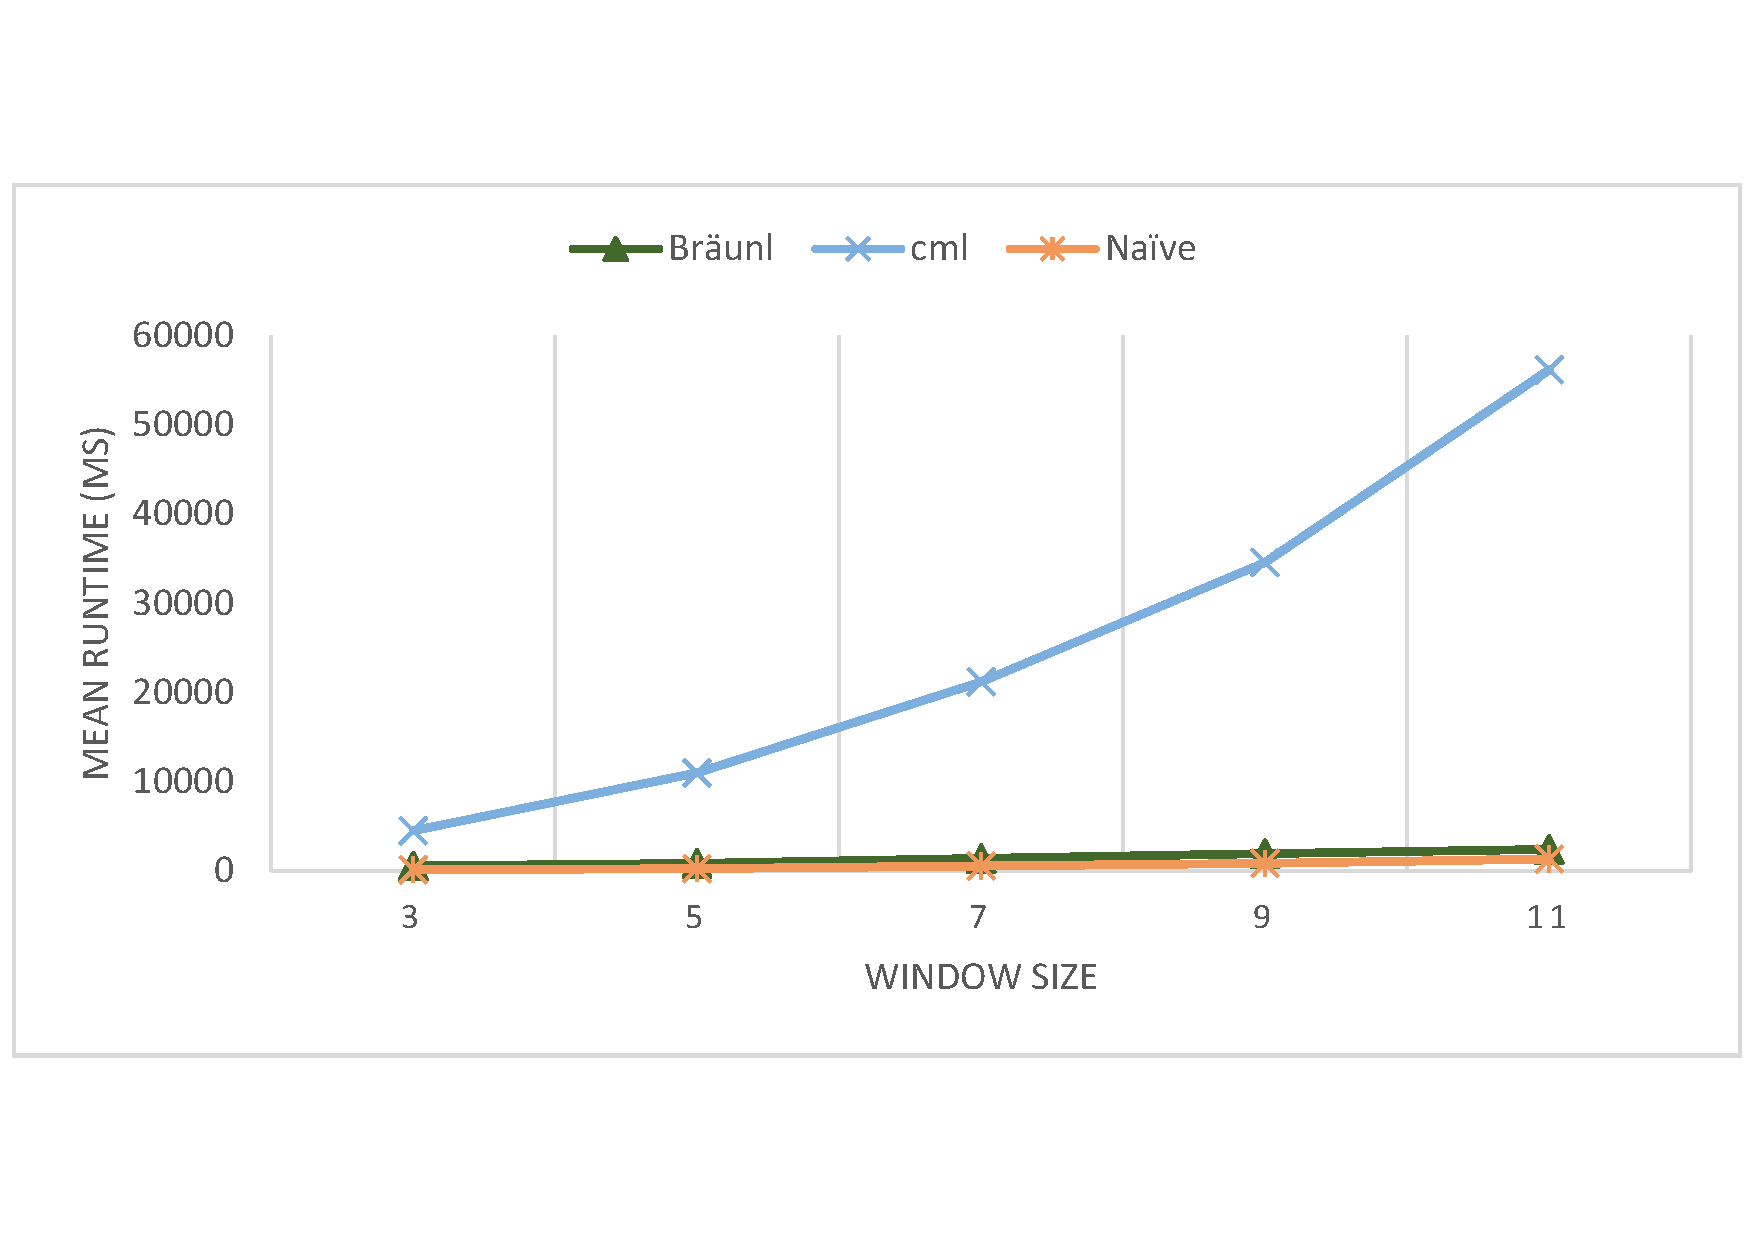
\includegraphics[width=0.5\textwidth]{images/charts/medium_chart}
% \caption{\label{graph:medium}Comparative graph of runtimes for medium image across window sizes}
% \end{figure}

%very small
\begin{figure}
\centering
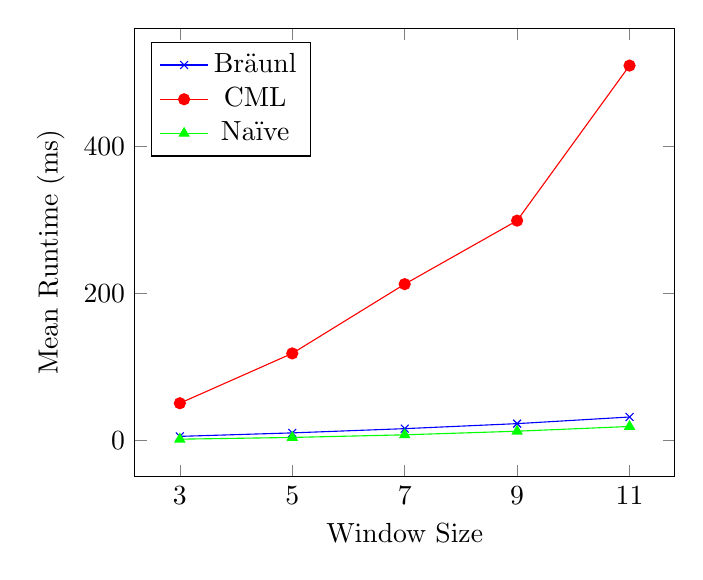
\begin{tikzpicture}
\begin{axis}[
	xlabel=Window Size,
    ylabel=Mean Runtime (ms),
    legend pos=north west,
    %xmin=3,
    %xmax=11,
    %minor x tick num=2,
    xtick=data
]
	\addplot [mark=x,blue] table [x=windowSize,y=Mean]{
    	Method	windowSize	filename	Mean	Error	StdDev	Median	Min	Scaled	ScaledSD	Gen0	Gen1	Gen2	Allocated
Bräunl	3	very-small	5.462	0.109	0.285	5.461	4.696	3.37	0.17	31.25	15.625	15.625	2.11
Bräunl	5	very-small	10.195	0.202	0.543	10.087	9.467	2.56	0.14	46.875	31.25	15.625	3.52
Bräunl	7	very-small	15.973	0.318	0.724	15.830	15.012	2.11	0.09	46.875	15.625	-	6.04
Bräunl	9	very-small	22.807	0.447	0.829	22.497	21.855	1.83	0.07	93.75	31.25	-	9.86
Bräunl	11	very-small	31.843	0.621	0.891	31.955	29.750	1.68	0.05	187.5	62.5	-	15.63


    };
    \addplot [mark=*,red] table [x=windowSize,y=Mean]{
    	Method	windowSize	filename	Mean	Error	StdDev	Median	Min	Scaled	ScaledSD	Gen0	Gen1	Gen2	Allocated
CML	3	very-small	50.588	2.544	7.500	49.480	40.127	31.18	4.6	166.6667	83.3333	-	1.68
CML	5	very-small	118.463	2.349	3.443	119.399	106.345	29.75	0.99	400	200	-	1.69
CML	7	very-small	212.817	7.252	21.270	220.862	152.973	28.08	2.79	1000	-	-	1.73
CML	9	very-small	299.339	5.264	4.396	298.044	296.011	23.98	0.34	2000	1000	-	1.83
CML	11	very-small	510.526	10.065	9.414	510.343	489.584	26.97	0.51	3000	1000	-	1.85

    };
    \addplot [mark=triangle*,green] table [x=windowSize,y=Mean]{
    	Method	windowSize	filename	Mean	Error	StdDev	Median	Min	Scaled	ScaledSD	Gen0	Gen1	Gen2	Allocated
Naïve	3	very-small	1.623	0.003	0.003	1.623	1.618	1	0	154.2969	35.1563	-	2.35
Naïve	5	very-small	3.983	0.076	0.071	3.980	3.891	1	0	382.8125	85.9375	-	5.62
Naïve	7	very-small	7.578	0.011	0.009	7.575	7.566	1	0	734.375	164.0625	-	10.52
Naïve	9	very-small	12.483	0.025	0.022	12.483	12.445	1	0	1171.875	203.125	-	17.26
Naïve	11	very-small	18.933	0.123	0.115	18.896	18.823	1	0	1718.75	187.5	-	23.9
    };
    
    \legend{Bräunl,CML,Naïve}
\end{axis}
\end{tikzpicture}
\caption{\label{graph:verysmall}Plot of mean runtimes for the very small size image}
\end{figure}

%peppers
\begin{figure}
\centering
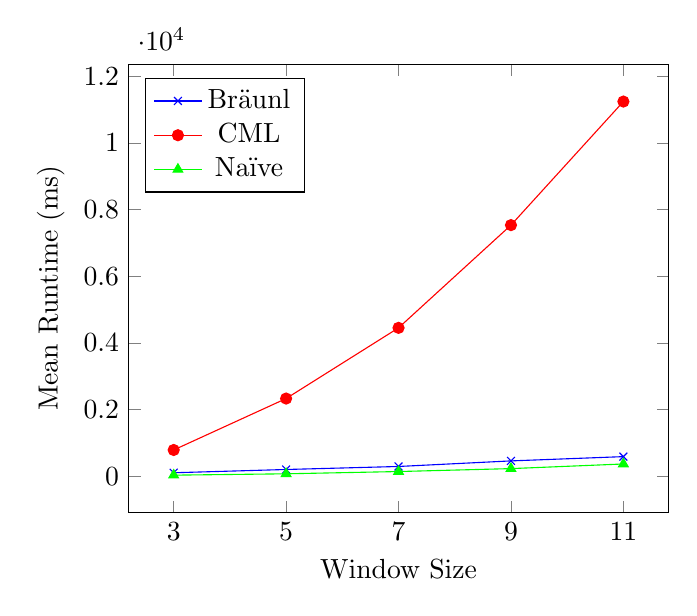
\begin{tikzpicture}
\begin{axis}[
	xlabel=Window Size,
    ylabel=Mean Runtime (ms),
    legend pos=north west,
    %xmin=3,
    %xmax=11,
    %minor x tick num=2,
    xtick=data
]
	\addplot [mark=x,blue] table [x=windowSize,y=Mean]{
    	Method	windowSize	filename	Mean	Error	StdDev	Median	Min	Scaled	ScaledSD	Gen0	Gen1	Gen2	Allocated
Bräunl	3	peppers_gray	108.436	2.141	5.088	108.817	93.931	2.98	0.18	1200	1000	1000	37.73
Bräunl	5	peppers_gray	206.336	4.112	9.693	205.430	187.900	2.68	0.15	1000	666.6667	666.6667	58.64
Bräunl	7	peppers_gray	296.717	5.718	5.616	297.432	286.169	2.05	0.12	2000	1000	1000	114.81
Bräunl	9	peppers_gray	463.857	9.138	8.975	464.704	449.199	2	0.13	3000	2000	1000	127.86
Bräunl	11	peppers_gray	592.056	11.749	21.483	589.079	557.281	1.62	0.21	5000	2000	1000	212.34

    };
    \addplot [mark=*,red] table [x=windowSize,y=Mean]{
    	Method	windowSize	filename	Mean	Error	StdDev	Median	Min	Scaled	ScaledSD	Gen0	Gen1	Gen2	Allocated
CML	3	peppers_gray	791.285	15.397	23.971	791.190	749.316	21.73	1.09	4000	2000	1000	28.14
CML	5	peppers_gray	2333.317	46.639	79.197	2339.807	2108.572	30.29	1.42	8000	3000	2000	28.67
CML	7	peppers_gray	4452.903	88.038	183.769	4407.427	4177.586	30.83	2.09	14000	5000	2000	28.28
CML	9	peppers_gray	7533.048	150.341	225.023	7527.491	7100.467	32.49	2.2	21000	7000	2000	28.29
CML	11	peppers_gray	11237.458	192.938	180.475	11266.773	10925.938	30.74	3.81	32000	10000	4000	29.38
    };
    \addplot [mark=triangle*,green] table [x=windowSize,y=Mean]{
    	Method	windowSize	filename	Mean	Error	StdDev	Median	Min	Scaled	ScaledSD	Gen0	Gen1	Gen2	Allocated
Naïve	3	peppers_gray	36.474	0.724	1.495	36.450	33.341	1	0	3357.1429	1000	1000	36.94
Naïve	5	peppers_gray	77.122	1.532	2.602	77.005	71.833	1	0	7285.7143	1000	1000	87.78
Naïve	7	peppers_gray	144.854	2.895	8.119	142.671	132.158	1	0	13750	1000	1000	175.21
Naïve	9	peppers_gray	232.750	5.198	15.245	227.335	213.438	1	0	21666.6667	1666.6667	1000	239.09
Naïve	11	peppers_gray	371.789	17.122	50.485	345.788	313.159	1	0	32000	1000	1000	337.86
    };
    
    \legend{Bräunl,CML,Naïve}
\end{axis}
\end{tikzpicture}
\caption{\label{graph:peppers}Plot of mean runtimes for the peppers image}
\end{figure}

%small
\begin{figure}
\centering
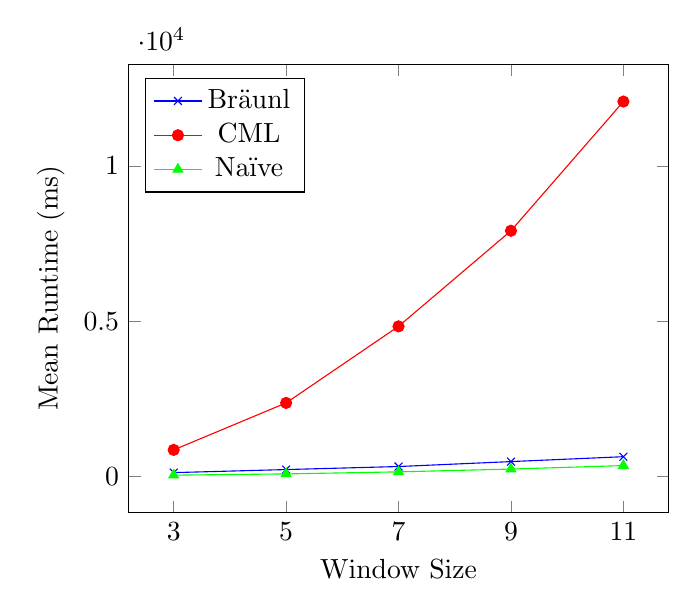
\begin{tikzpicture}
\begin{axis}[
	xlabel=Window Size,
    ylabel=Mean Runtime (ms),
    legend pos=north west,
    %xmin=3,
    %xmax=11,
    %minor x tick num=2,
    xtick=data
]
	\addplot [mark=x,blue] table [x=windowSize,y=Mean]{
    	Method	windowSize	filename	Mean	Error	StdDev	Median	Min	Scaled	ScaledSD	Gen0	Gen1	Gen2	Allocated
Bräunl	3	small	116.782	2.334	4.208	116.874	107.437	3.32	0.14	1200	1000	800	40.96
Bräunl	5	small	215.573	4.295	12.185	217.475	180.880	2.86	0.16	1666.6667	1333.3333	1000	63.03
Bräunl	7	small	313.114	2.952	2.761	312.674	309.410	2.21	0.02	2000	1000	1000	111.37
Bräunl	9	small	472.517	4.680	4.378	473.456	460.456	2.04	0.02	4000	2000	1000	161.63
Bräunl	11	small	629.898	5.558	4.927	628.729	618.231	1.83	0.02	5000	2000	1000	149.05

    };
    \addplot [mark=*,red] table [x=windowSize,y=Mean]{
    	Method	windowSize	filename	Mean	Error	StdDev	Median	Min	Scaled	ScaledSD	Gen0	Gen1	Gen2	Allocated
CML	3	small	849.482	19.570	56.149	828.209	773.390	24.12	1.69	4000	2000	1000	33.68
CML	5	small	2362.643	46.461	104.871	2355.982	2162.910	31.39	1.39	9000	3000	2000	33.25
CML	7	small	4830.294	95.856	137.474	4834.632	4523.971	34.15	0.97	14000	5000	2000	33.04
CML	9	small	7910.925	134.530	125.839	7909.106	7701.102	34.15	0.54	23000	8000	3000	34.13
CML	11	small	12074.170	232.388	228.236	12042.342	11712.425	35.17	0.66	32000	11000	3000	34

    };
    \addplot [mark=triangle*,green] table [x=windowSize,y=Mean]{
    	Method	windowSize	filename	Mean	Error	StdDev	Median	Min	Scaled	ScaledSD	Gen0	Gen1	Gen2	Allocated
Naïve	3	small	35.246	0.697	0.881	34.905	34.267	1	0	3466.6667	1000	1000	37.65
Naïve	5	small	75.282	0.506	0.473	75.217	74.419	1	0	7857.1429	1000	1000	95.36
Naïve	7	small	141.432	0.804	0.752	141.446	140.203	1	0	14000	1000	1000	175.74
Naïve	9	small	231.667	0.979	0.867	232.029	229.561	1	0	22666.6667	1666.6667	1000	328.08
Naïve	11	small	343.286	1.710	1.600	342.643	341.541	1	0	33000	1000	1000	261.29
    };
    
    \legend{Bräunl,CML,Naïve}
\end{axis}
\end{tikzpicture}
\caption{\label{graph:small}Plot of mean runtimes for the small size image}
\end{figure}

%medium
\begin{figure}
\centering
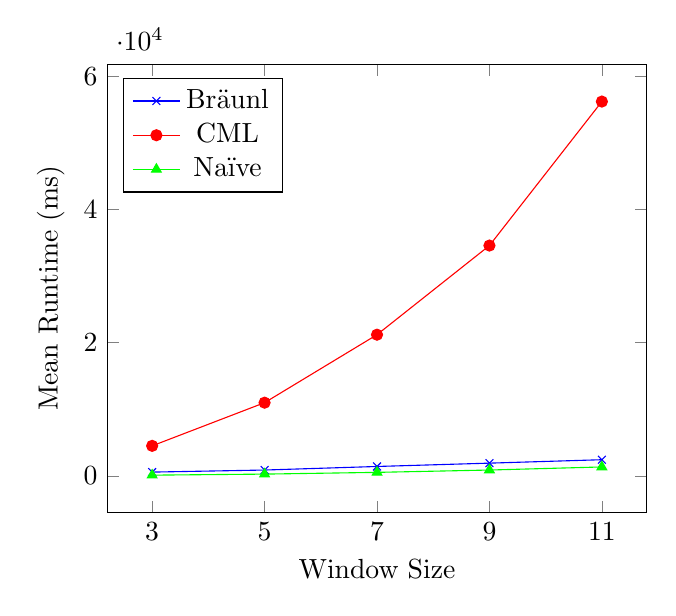
\begin{tikzpicture}
\begin{axis}[
	xlabel=Window Size,
    ylabel=Mean Runtime (ms),
    legend pos=north west,
    %xmin=3,
    %xmax=11,
    %minor x tick num=2,
    xtick=data
]
	\addplot [mark=x,blue] table [x=windowSize,y=Mean]{
    	Method	windowSize	filename	Mean	Error	StdDev	Median	Min	Scaled	ScaledSD	Gen0	Gen1	Gen2	Allocated
Bräunl	3	medium	589.431	11.668	10.344	585.135	574.774	4.51	0.27	2000	1000	1000	146.49
Bräunl	5	medium	899.233	4.445	3.940	899.270	892.109	3.12	0.07	4000	2000	1000	230.3
Bräunl	7	medium	1433.220	31.164	29.151	1431.262	1379.761	2.61	0.07	7000	4000	2000	374.04
Bräunl	9	medium	1933.758	24.222	22.657	1925.642	1905.768	2.15	0.02	16000	4000	2000	527.35
Bräunl	11	medium	2447.284	47.271	50.580	2451.473	2352.536	1.8	0.05	40000	4000	2000	167.19

    };
    \addplot [mark=*,red] table [x=windowSize,y=Mean]{
    	Method	windowSize	filename	Mean	Error	StdDev	Median	Min	Scaled	ScaledSD	Gen0	Gen1	Gen2	Allocated
CML	3	medium	4527.962	89.754	226.819	4511.961	4003.316	34.65	2.61	12000	6000	3000	132.41
CML	5	medium	11006.775	197.445	184.691	10983.829	10737.131	38.19	1.05	28000	10000	4000	138.84
CML	7	medium	21210.296	417.303	409.847	21118.240	20410.160	38.61	1.08	50000	15000	4000	136.78
CML	9	medium	34587.347	471.655	441.186	34687.611	33898.247	38.45	0.48	81000	22000	4000	137.63
CML	11	medium	56196.611	1118.853	2548.193	55158.372	52956.449	41.29	2.05	230000	66000	4000	132.75
    };
    \addplot [mark=triangle*,green] table [x=windowSize,y=Mean]{
    	Method	windowSize	filename	Mean	Error	StdDev	Median	Min	Scaled	ScaledSD	Gen0	Gen1	Gen2	Allocated
Naïve	3	medium	131.111	2.655	7.787	128.188	122.294	1	0	11500	1500	1500	102.34
Naïve	5	medium	288.343	5.716	6.805	285.656	282.623	1	0	28000	1000	1000	371.43
Naïve	7	medium	549.600	12.951	12.114	543.465	539.418	1	0	54000	1000	1000	710.4
Naïve	9	medium	899.563	3.131	2.444	900.523	893.992	1	0	89000	2000	1000	985.29
Naïve	11	medium	1361.629	27.108	31.217	1350.193	1344.088	1	0	131000	4000	1000	1969.78
    };
    
    \legend{Bräunl,CML,Naïve}
\end{axis}
\end{tikzpicture}
\caption{\label{graph:medium}Plot of mean runtimes for the medium size image}
\end{figure}

%CML
\begin{figure}
\centering
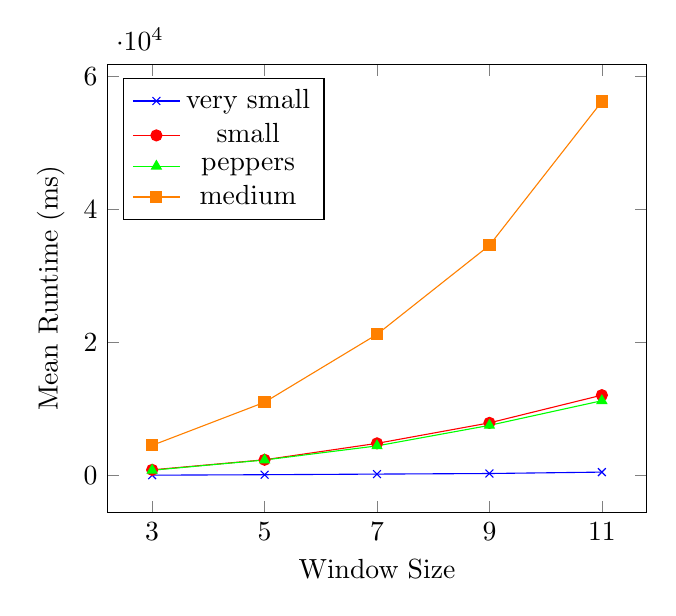
\begin{tikzpicture}
\begin{axis}[
	xlabel=Window Size,
    ylabel=Mean Runtime (ms),
    legend pos=north west,
    %xmin=3,
    %xmax=11,
    %minor x tick num=2,
    xtick=data
]
	\addplot [mark=x,blue] table [x=windowSize,y=Mean]{
    	Method	windowSize	filename	Mean	Error	StdDev	Median	Min	Scaled	ScaledSD	Gen0	Gen1	Gen2	Allocated
CML	3	very-small	50.588	2.544	7.500	49.480	40.127	31.18	4.6	166.6667	83.3333	-	1.68
CML	5	very-small	118.463	2.349	3.443	119.399	106.345	29.75	0.99	400	200	-	1.69
CML	7	very-small	212.817	7.252	21.270	220.862	152.973	28.08	2.79	1000	-	-	1.73
CML	9	very-small	299.339	5.264	4.396	298.044	296.011	23.98	0.34	2000	1000	-	1.83
CML	11	very-small	510.526	10.065	9.414	510.343	489.584	26.97	0.51	3000	1000	-	1.85


    };
    \addplot [mark=*,red] table [x=windowSize,y=Mean]{
    	Method	windowSize	filename	Mean	Error	StdDev	Median	Min	Scaled	ScaledSD	Gen0	Gen1	Gen2	Allocated
CML	3	small	849.482	19.570	56.149	828.209	773.390	24.12	1.69	4000	2000	1000	33.68
CML	5	small	2362.643	46.461	104.871	2355.982	2162.910	31.39	1.39	9000	3000	2000	33.25
CML	7	small	4830.294	95.856	137.474	4834.632	4523.971	34.15	0.97	14000	5000	2000	33.04
CML	9	small	7910.925	134.530	125.839	7909.106	7701.102	34.15	0.54	23000	8000	3000	34.13
CML	11	small	12074.170	232.388	228.236	12042.342	11712.425	35.17	0.66	32000	11000	3000	34

    };
    \addplot [mark=triangle*,green] table [x=windowSize,y=Mean]{
    	Method	windowSize	filename	Mean	Error	StdDev	Median	Min	Scaled	ScaledSD	Gen0	Gen1	Gen2	Allocated
CML	3	peppers_gray	791.285	15.397	23.971	791.190	749.316	21.73	1.09	4000	2000	1000	28.14
CML	5	peppers_gray	2333.317	46.639	79.197	2339.807	2108.572	30.29	1.42	8000	3000	2000	28.67
CML	7	peppers_gray	4452.903	88.038	183.769	4407.427	4177.586	30.83	2.09	14000	5000	2000	28.28
CML	9	peppers_gray	7533.048	150.341	225.023	7527.491	7100.467	32.49	2.2	21000	7000	2000	28.29
CML	11	peppers_gray	11237.458	192.938	180.475	11266.773	10925.938	30.74	3.81	32000	10000	4000	29.38
    };
    \addplot [mark=square*,orange] table [x=windowSize,y=Mean]{
    	Method	windowSize	filename	Mean	Error	StdDev	Median	Min	Scaled	ScaledSD	Gen0	Gen1	Gen2	Allocated
CML	3	medium	4527.962	89.754	226.819	4511.961	4003.316	34.65	2.61	12000	6000	3000	132.41
CML	5	medium	11006.775	197.445	184.691	10983.829	10737.131	38.19	1.05	28000	10000	4000	138.84
CML	7	medium	21210.296	417.303	409.847	21118.240	20410.160	38.61	1.08	50000	15000	4000	136.78
CML	9	medium	34587.347	471.655	441.186	34687.611	33898.247	38.45	0.48	81000	22000	4000	137.63
CML	11	medium	56196.611	1118.853	2548.193	55158.372	52956.449	41.29	2.05	230000	66000	4000	132.75
    };
    
    \legend{very small,small,peppers,medium}
\end{axis}
\end{tikzpicture}
\caption{\label{graph:cmls}Plot of mean runtimes for the CML algorithm on different images sizes}
\end{figure}

\begin{figure*}
% \subfloat[]{\includegraphics[width=0.2\textwidth]{chatpers/medianfilter/images/peppers/peppers_gray.png}}
% \subfloat[]{\includegraphics[width=0.2\textwidth]{chatpers/medianfilter/images/peppers/peppers_gray_noisy.png}}
% \subfloat[]{\includegraphics[width=0.2\textwidth]{chatpers/medianfilter/images/peppers/naive_peppers_gray_noisy_3.png}}
% \subfloat[]{\includegraphics[width=0.2\textwidth]{chatpers/medianfilter/images/peppers/braunl_peppers_gray_noisy_3.png}}
% \subfloat[]{\includegraphics[width=0.2\textwidth]{chatpers/medianfilter/images/peppers/cml_peppers_gray_noisy_3.png}}
\subfloat[]{\includegraphics[width=0.2\textwidth]{chapters/medianfilter/images/peppers/peppers_gray.png}}
\subfloat[]{\includegraphics[width=0.2\textwidth]{chapters/medianfilter/images/peppers/peppers_gray_noisy.png}}
\subfloat[]{\includegraphics[width=0.2\textwidth]{chapters/medianfilter/images/peppers/naive_peppers_gray_noisy_3.png}}
\subfloat[]{\includegraphics[width=0.2\textwidth]{chapters/medianfilter/images/peppers/braunl_peppers_gray_noisy_3.png}}
\subfloat[]{\includegraphics[width=0.2\textwidth]{chapters/medianfilter/images/peppers/cml_peppers_gray_noisy_3.png}}
\caption{\label{fig:peppers}The classic grayscale `peppers' image, before and after processing.  (a) is the original image; (b) is the image with random salt \& pepper noise introduced; (c) is the result of processing the image using the na\"{i}ve algorithm; (d) is the result of processing the image using the Br\"{a}unl-inspired algorithm; (e) is the result of processing the image using the CML algorithm}
\end{figure*}

% Please add the following required packages to your document preamble:
% \usepackage{booktabs}
\begin{table}
\centering
\caption{Peak signal-to-noise ratio measurement for the very small image (measured in dB)}
\label{tab:psnrvsmall}
\begin{tabular}{@{}lccccc@{}}
\toprule
\multicolumn{1}{c}{\textbf{Algorithm}} & \multicolumn{5}{c}{\textbf{Window size}}                                          \\
                                       & 3              & 5              & 7              & 9             & 11             \\ \midrule
Bräunl                                 & 20.78          & 17.82          & 15.65          & 14.36         & 13.55          \\
CML                                    & 25.98          & \textbf{21.85} & \textbf{18.62} & \textbf{16.40} & 14.99          \\
Naïve                                  & \textbf{27.03} & 21.74          & 18.55          & 16.39         & \textbf{15.02} \\ \bottomrule
\end{tabular}
\end{table}

% Please add the following required packages to your document preamble:
% \usepackage{booktabs}
\begin{table}
\centering
\caption{Peak signal-to-noise ratio measurement for the peppers image (measured in dB)}
\begin{tabular}{@{}lccccc@{}}
\toprule
\multicolumn{1}{c}{\textbf{Algorithm}} & \multicolumn{5}{c}{\textbf{Window size}}                                          \\
                                       & 3              & 5              & 7              & 9              & 11            \\ \midrule
Bräunl                                 & 28.76          & 27.35          & 25.27          & 23.94          & 22.82         \\
CML                                    & 31.85          & 31.07          & 29.8           & 28.56          & 27.42         \\
Naïve                                  & \textbf{32.79} & \textbf{31.25} & \textbf{29.87} & \textbf{28.63} & \textbf{27.50} \\ \bottomrule
\end{tabular}
\label{tab:psnrpeppers}
\end{table}

% Please add the following required packages to your document preamble:
% \usepackage{booktabs}
\begin{table}
\centering
\caption{Peak signal-to-noise ratio measurement for the small image (measured in dB)}
\label{tab:psnrsmall}
\begin{tabular}{@{}lccccc@{}}
\toprule
\multicolumn{1}{c}{\textbf{Algorithm}} & \multicolumn{5}{c}{\textbf{Window size}}                                          \\
                                       & 3              & 5              & 7             & 9              & 11             \\ \midrule
Bräunl                                 & 32.83          & 32.34          & 30.74         & 29.73          & 28.94          \\
CML                                    & 36.62          & 34.25          & 32.66         & 31.57          & 30.71          \\
Naïve                                  & \textbf{37.83} & \textbf{34.31} & \textbf{32.7} & \textbf{31.65} & \textbf{30.81} \\ \bottomrule
\end{tabular}
\end{table}

% Please add the following required packages to your document preamble:
% \usepackage{booktabs}
\begin{table}
\centering
\caption{Peak signal-to-noise ratio measurement for the medium image (measured in dB)}
\begin{tabular}{@{}lccccc@{}}
\toprule
\multicolumn{1}{c}{\textbf{Algorithm}} & \multicolumn{5}{c}{\textbf{Window size}}                                           \\
                                       & 3              & 5              & 7              & 9              & 11             \\ \midrule
Bräunl                                 & 32.98          & 32.65          & 31.59          & 30.91          & 30.36          \\
CML                                    & 36.72          & \textbf{34.15} & \textbf{32.98} & \textbf{32.26} & \textbf{31.73} \\
Naïve                                  & \textbf{37.16} & 34.07          & 32.96          & \textbf{32.26} & \textbf{31.73} \\ \bottomrule
\end{tabular}
\label{tab:psnrmedium}
\end{table}

Examination of the reported memory statistics (please see the GitHub repository for details) appears to show that the maximum amount of memory allocated during processing for the CML algorithm stays roughly constant across window sizes for each image size, and in fact on larger window sizes it is the most memory efficient.  The naïve algorithm quickly grows to consume the most memory at larger window sizes for each image size, suggesting that it likely derives some of its comparative speed at the cost of greater space complexity, while Bräunl sits in the middle.  Conversely, CML generates by far the most garbage collection events, which may well go some way to explaining its relative lack of pace.

\section{Discussion}
%These algorithms are not necessarily the best for performing this operation, as they ignore the potential for taking advantage of data-parallelism.

The algorithms developed and presented here are not necessarily optimal for the purpose.  They largely handle each pixel separately, or combine them into arrays on-the-fly.  This ignores the possibility of exploiting data-parallelism to improve throughput, and instead relies only on the separate CPU cores to provide the parallelism.  %Unfortunately, a lack of time prevented further exploration of this.  .NET Core provides relatively little support for CPU vector instructions anyway.

%It is unclear how much any of the given approaches attempts to exploit the processor cache.

It is unclear how much the mechanics underlying these implementations (i.e. the .NET Core and \hopac{} systems) attempt to maximise use of the processor cache.  Efficient use of the cache can contribute significantly to an optimised version of an algorithm outperforming a simplistic version by an order of magnitude or more \cite{Ragan-Kelley2017}.  No attempt was made manually to ensure good practices such as tiling or striping.  %Differences in cache exploitation may also go some way to explaining differences in execution time.

The CML approach used essentially instantiates a separate logical processing element for each pixel, each of which must be scheduled to run at some point -- concurrent with another one in the case of synchronous message passing.  It is possible that this surfeit of separate logical threads may induce excessive switching costs, and perhaps promote wasted time with threads spending time polling their channel and their neighbours'.  Careful improvements to this and the use of the cache could perhaps lead to significant gains in speed.

In terms of the code itself also, CML appears to be the worst.  The program requires roughly double the number of lines of the naïve program, and is arguably much less `clean' or `readable'.  Reinterpreting the median filter in terms of synchronously communicating processes has not yielded a structural improvement nor simplified the programming task.  Combined with the running time results above, this suggests that the CML approach is actively unhelpful for implementing MWTs, at least when using \hopac{}.  %While potentially not as important as execution speed or peak memory use, code that is difficult to comprehend is difficult to maintain and more prone to non-obvious bugs.  This seems to be a further weakness of the CML style as applied to MWTs.

Basic profiling of the CML-based implementation appears to indicate that more than half of the runtime of the program was spent inside the function for giving a value over a channel, and functions called by it.  Furthermore, according to this profiling, almost 40\% of the total running time of the algorithm is taken up specifically by low-level memory management functions inside the depths of the .NET Core system.  Considering that some of these functions are written in hand-optimised assembly, the fact they account for so much of the running time appears to suggest that memory use is poorly handled in the tested implementation.

MWTs are generally relatively simplistic processes, which typically consist simply of combining values from the pixel array, which can be programmed in a straightforward fashion.  More sophisticated programming techniques may simply `get in the way' and introduce unnecessary overheads, which appears to have happened here.  Furthermore, the median filter can largely be broken down into arithmetic and logical operations amenable to vectorisation (e.g. \cite{Sanchez2012,Perreault2007}), which the CML approach (currently, at least) ignores entirely.

\subsection{Threats to validity}
There are two identifiable threats to validity, both regarding the `quality' of the programming involved.  .NET Core, as a widely used open source compiler and runtime system which has likely had millions of man-hours invested in it, is presumably of high quality and fast in most cases.  That is not necessarily the case with \hopac{}.  While it is open source, and moderately well-known in the F\# community, the amount of time spent on optimising it is likely nowhere close to that spent on .NET Core.  This means that \hopac{} itself may present significant bottlenecks in the course of performing the MWT.  While it is reasonable to expect that `give' operations would be a large part of the total running time, as a central part of the operation of the algorithm, it is surprising to see it take more than 50\% of the time.

The other threat to validity is the skill of the end programmer.  The author was new to the \hopac{} library at the start of this work, and inferior design choices have may been made unwittingly.  It was, however, suggested in the course of personal communication with one of the maintainers and fellow users of the \hopac{} library that the CML approach may simply be a poor fit to pixel-wise image processing tasks.

Fundamentally, the results achieved here, as with most implementation exercises, succeed or fail in large part on the skill, knowledge and effort of the programmers involved.  The use of other libraries may lead to better results.  Other relatively recent implementations of CML exist, such as Concurrent Haskell \cite{Chaudhuri2009} and Fibers\footnote{\url{https://github.com/wingo/fibers}} for Guile Scheme, but a lack of time meant that they could not yet be assessed further.

\section{Conclusion}
The use of a Concurrent ML approach to image processing was explored in this work, in particular as applied to the median filter MWT operation.  The measured results suggest that it is much worse than using a simple naïve nested for-loop approach.  The reason for this appears to be primarily related to overhead from the synchronous communications, especially with regards to memory allocations and garbage collections.  This may be an issue with the CML style in general, or it may be an issue related to the CML library used or the programming of the algorithms tested here.  More work is required to determine this for certain.  CML does appear to provide one advantage, however, in that for larger window sizes it seemingly has the lowest peak space requirement.

A CML approach where a separate logical processing element is used to represent each pixel largely eliminates the possibility of taking advantage of data-parallel hardware, such as vector instructions of CPUs or GPUs.  For situations where vector instructions are applicable, the CML approach seems likely to be a poor choice.  It is not clear, however, how well this approach may or may not work for instances where the data types involved are more complex, or where there is a significant level of control flow involved.

Future work should explore CML as applied to other computer vision algorithms, especially those which can naturally be characterised in terms of message passing, or which use more complex data types.  Other CML implementations beyond the one used here should be tested too, as it is not clear how much the problems experienced by this CML program may stem from the implementation of the CML library used.



% if have a single appendix:
%\appendix[Proof of the Zonklar Equations]
% or
%\appendix  % for no appendix heading
% do not use \section anymore after \appendix, only \section*
% is possibly needed

% use appendices with more than one appendix
% then use \section to start each appendix
% you must declare a \section before using any
% \subsection or using \label (\appendices by itself
% starts a section numbered zero.)
%


% \appendices
% \section{Proof of the First Zonklar Equation}
% Appendix one text goes here.

% % you can choose not to have a title for an appendix
% % if you want by leaving the argument blank
% \section{}
% Appendix two text goes here.


% % use section* for acknowledgment
% \section*{Acknowledgments}
% The author would like to thank the creators and maintainers of the open source .NET libraries \hopac{}, ImageSharp and BenchmarkDotNet, all three of which were used in the preparation of this paper, for their time and efforts.  Particular thanks is given to Anton Firsov of the ImageSharp team, for assistance with correct use of the API.  The author would also like to thank Pexels.com and its contributing photographers, for making the images used in this paper freely available.

% Thanks must also go to the anonymous reviewers, who's feedback and suggestions did much to improve this paper.


% % Can use something like this to put references on a page
% % by themselves when using endfloat and the captionsoff option.
% \ifCLASSOPTIONcaptionsoff
%   \newpage
% \fi



% trigger a \newpage just before the given reference
% number - used to balance the columns on the last page
% adjust value as needed - may need to be readjusted if
% the document is modified later
%\IEEEtriggeratref{8}
% The "triggered" command can be changed if desired:
%\IEEEtriggercmd{\enlargethispage{-5in}}

% references section

% can use a bibliography generated by BibTeX as a .bbl file
% BibTeX documentation can be easily obtained at:
% % http://mirror.ctan.org/biblio/bibtex/contrib/doc/
% % The IEEEtran BibTeX style support page is at:
% % http://www.michaelshell.org/tex/ieeetran/bibtex/
% \bibliographystyle{IEEEtran}
% % argument is your BibTeX string definitions and bibliography database(s)
% %\bibliography{IEEEabrv,../bib/biblio}
% \bibliography{bibtex/bib/biblio.bib}
%
% <OR> manually copy in the resultant .bbl file
% set second argument of \begin to the number of references
% (used to reserve space for the reference number labels box)
% \begin{thebibliography}{1}

% \bibitem{IEEEhowto:kopka}
% H.~Kopka and P.~W. Daly, \emph{A Guide to \LaTeX}, 3rd~ed.\hskip 1em plus
%   0.5em minus 0.4em\relax Harlow, England: Addison-Wesley, 1999.

% \end{thebibliography}

% % biography section
% % 
% % If you have an EPS/PDF photo (graphicx package needed) extra braces are
% % needed around the contents of the optional argument to biography to prevent
% % the LaTeX parser from getting confused when it sees the complicated
% % \includegraphics command within an optional argument. (You could create
% % your own custom macro containing the \includegraphics command to make things
% % simpler here.)
% %\begin{IEEEbiography}[{\includegraphics[width=1in,height=1.25in,clip,keepaspectratio]{mshell}}]{Michael Shell}
% % or if you just want to reserve a space for a photo:

% \begin{IEEEbiography}{Michael Shell}
% Biography text here.
% \end{IEEEbiography}

% % if you will not have a photo at all:
% \begin{IEEEbiographynophoto}{John Doe}
% Biography text here.
% \end{IEEEbiographynophoto}

% % insert where needed to balance the two columns on the last page with
% % biographies
% %\newpage

% \begin{IEEEbiographynophoto}{Jane Doe}
% Biography text here.
% \end{IEEEbiographynophoto}

% You can push biographies down or up by placing
% a \vfill before or after them. The appropriate
% use of \vfill depends on what kind of text is
% on the last page and whether or not the columns
% are being equalized.

%\vfill

% Can be used to pull up biographies so that the bottom of the last one
% is flush with the other column.
%\enlargethispage{-5in}



% that's all folks
% \end{document}


